% ****** Start of file aipsamp.tex ******
%
%   This file is part of the AIP files in the AIP distribution for REVTeX 4.
%   Version 4.1 of REVTeX, October 2009
%
%   Copyright (c) 2009 American Institute of Physics.

% Use this file as a source of example code for your aip document.
% Use the file aiptemplate.tex as a template for your document.
\documentclass[%
 aip,
 jmp,%
 amsmath,amssymb,
%preprint,%
 reprint,%
%author-year,%
%author-numerical,%
]{revtex4-1}

\usepackage{graphicx}% Include figure files
\usepackage{grffile}
\usepackage{dcolumn}% Align table columns on decimal point
\usepackage{bm}% bold math
%\usepackage[mathlines]{lineno}% Enable numbering of text and display math
%\linenumbers\relax % Commence numbering lines
\usepackage{multirow}
\usepackage{color} % for the notes
\usepackage{etex}
\reserveinserts{58}
\usepackage{morefloats}

%%%%%%%%%%%%
\usepackage{listings}
\usepackage{xcolor}       
\definecolor{dkgreen}{rgb}{0,0.6,0}
\definecolor{gray}{rgb}{0.5,0.5,0.5}
\definecolor{light-gray}{rgb}{0.97,0.97,0.97}

\lstdefinelanguage{owlms}
    {morekeywords={xsd,owl,xml,dc,rdf,skos,description,PlainLiteral,int,float,
        some,only,value,min,exactly,max,and,or,not,
        Prefix,Ontology,Import,Individual,Facts,Types,Class,
        DataProperty,ObjectProperty,AnnotationProperty,Annotations,
        DifferentIndividuals,SubClassOf,EquivalentTo,DisjointWith,DisjointUnionOf,SubPropertyOf,DisjointClasses,DisjointProperties,
        Symmetric,Asymmetric,Reflexive,Irreflexive,Transitive,Functional,InverseFunctional,
        Characteristics,Range,Domain,Datatype},
     basicstyle=\scriptsize\ttfamily,
     backgroundcolor=\color{light-gray},
     keywordstyle=\color{blue},
     commentstyle=\color{gray},
     stringstyle=\color{dkgreen},
     numbers=left,
     numberstyle=\tiny\color{gray},
     stepnumber=1,
     numbersep=10pt,
     tabsize=2,
     showspaces=false,
     showstringspaces=false,
     breaklines=true,                           % wrap text
     sensitive=true,                            % keywords are case sensitive
     morecomment=[l][commentstyle]{\#},         % comment format
     morestring=[b]",                           % string format
literate=%
  {ã}{{\~a}}1
  {â}{{\^a}}1
  {õ}{{\~o}}1
  {á}{{\'a}}1
  {ú}{{\'u}}1
  {í}{{\'i}}1
  {é}{{\'e}}1
  {Ç}{{\c{C}}}1
  {Õ}{{\~O}}1
  {Ê}{{\^E}}1
  {ó}{{\'o}}1
  {à}{{\`a}}1
  {Â}{{\^A}}1
  {ô}{{\^o}}1
  {ê}{{\^e}}1
  {ç}{{\c{c}}}1
}


\begin{document}

\preprint{XXXXX (preprint)}

\title[Ontology of Social Participation (OSP)]{Ontology of Social Participation: Community Documentation, Expansion and Examples of Use}% Force line breaks with \\

\author{Renato Fabbri}%
 \homepage{http://ifsc.usp.br/~fabbri/}
 \email{fabbri@usp.br}
  \affiliation{ 
Instituto de F\'isica de S\~ao Carlos, Universidade de S\~ao Paulo (IFSC/USP)%\\This line break forced with \textbackslash\textbackslash
}%

\author{Henrique Parra Parra Filho}
  \homepage{http://www.cidadedemocratica.org.br/}
  \email{henrique@cidadedemocratica.org.br}
 \altaffiliation{Cidade Democr\'atica}%Lines break automatically or can be forced with \\

\author{Rodrigo Bandeira de Luna}
  \homepage{http://www.cidadedemocratica.org.br/}
  \email{rodrigoyellow@cidadedemocratica.org.br}
 \altaffiliation{Cidade Democr\'atica}%Lines break automatically or can be forced with \\
%
%\author{Vilson Vieira da Silva Junior}
%  \homepage{http://automata.cc/}
%  \email{vilson@void.cc}
%  \altaffiliation[Also at ]{IFSC-USP}%Lines break automatically or can be forced with \\
%
%\author{Ricardo Fabbri}
%  \homepage{http://www.lems.brown.edu/~rfabbri/}
%  \email{rfabbri@iprj.uerj.br}
% \altaffiliation{
%Instituto Polit\'ecnico, Universidade Estadual do Rio de Janeiro (IPRJ)
%}%Lines break automatically or can be forced with \\
%
%\author{Deborah Christina Antunes}
%  \homepage{http://lattes.cnpq.br/1065956470701739}
%  \email{deborahantunes@gmail.com}
%  \altaffiliation{
%Curso de Psicologia, Universidade Federal do Cer\'a (UFC - Sobral)
%}%Lines break automatically or can be forced with \\
%
%\author{Marilia Mello Pisani}
%  \homepage{http://lattes.cnpq.br/6738980149860322}
%  \email{marilia.m.pisani@gmail.com}
% \altaffiliation{
%Centro de Ci\^encias Naturais e Humanas, Universidade Federal do ABC (CCNH/UFABC)
%}
%
%\author{Luciano da Fontoura Costa}
%  \homepage{http://cyvision.ifsc.usp.br/~luciano/}
%  \email{ldfcosta@gmail.com}
%  \altaffiliation[Also at ]{IFSC-USP}%Lines break automatically or can be forced with \\
%
%\author{Ricardo Augusto Poppi Martins}
%  \homepage{http://ricardopoppi.wordpress.com/}
%  \email{ricardo.poppi@presidencia.gov.br}
% \altaffiliation{Secretaria-Geral da Presidência da República (SG/PR)}%Lines break automatically or can be forced with \\
%
%\author{Ronald Emerson Scherolt da Costa}
%  \homepage{http://www.icmc.usp.br/pessoas/dilvan/}
%  \email{ronald.costa@presidencia.gov.br}
% \altaffiliation[Also at ]{SG/PR}%Lines break automatically or can be forced with \\
%
%
%\author{Osvaldo Novais de Oliveira Junior}
%  \homepage{www.polimeros.ifsc.usp.br/professors/professor.php?id=4}
%  \email{chu@ifsc.usp.br}
% \altaffiliation[Also at ]{IFSC-USP}%Lines break automatically or can be forced with \\
%

\author{Flor Karina Mamani Amanqui}
  \homepage{http://java.icmc.usp.br}
  \email{florkarina27@gmail.com}
 \altaffiliation{Instituto de Ci\^encias Matemáticas e de Computação (ICMC/USP)}%Lines break automatically or can be forced with \\



\author{Dilvan A. Moreira}
  \homepage{http://java.icmc.usp.br}
  \email{dilvan@icmc.usp.br}
 \altaffiliation[also at ]{(ICMC/USP)}%Lines break automatically or can be forced with \\





\date{\today}% It is always \today, today,
             %  but any date may be explicitly specified

\begin{abstract}
Participatory democracy advances in virtually all governments. South America presents a prominent context with mixed culture and social predisposition. At 2012, civil, academic and governmental parties started elaborating the ``Common Vocabulary of Social Participation'' (CVSP), as a public and online process. By May, 2013, first reference documents were online, together with a preliminary OWL code,
logos, and a diagram of a general ``public consultation''.
To ease this process, the Corais platform was used, which kept online records of the process, like discussions and preparation of texts. 
This article exposes this material and proposes elementary unfolding, including the ``Ontology of Social Participation'' (OSP). To exhibit this new ontology, this steps were considered: completion of CVSP OWL code for current OSP, with necessary translations and corrections; an expansion of the ontology by further specifying classes; finally, use examples regarding knowledge organization and a SparQL endpoint. Further work involves association with the social participation federal portal from Brazil,
expansion to a more structured participation artifact, and careful consideration of upper ontologies such as BFO and DBpedia.
\end{abstract}

\pacs{89.65-s,07.05.Kf}% PACS, the Physics and Astronomy
\keywords{OWL, electronic government, electronic democracy, participatory democracy, semantic web, linked data, social network analysis}%Use showkeys class option if keyword
\maketitle


\section{Introduction}\label{sec:into}
Easy access to social media is reshaping citizen participation in government affairs~\cite{socMed}.
Information and communication technologies (ICTs) have exhibited such an impact on the way individuals interact
 that it is giving birth to new organizational methods to social movements, like the 2010 Arab Spring and the 2013 Brazilian protests. These events gathered millions of people and, although recent, have shown direct and strong impact in governments and new laws, and the forecast is an intensification of the process~\cite{digRev1,digRev2,digRev3}.

Concomitantly, electronic government initiatives are flourishing. Favored mainly by the ubiquity of Internet technologies (e.g. Web 2.0, HTML 5, open source browsers, etc.) and by the need for renewal of representative democracy practices. 
These initiatives have taken place in various platforms, including usual social networks (e.g. Facebook, Tweeter, etc)
 and dedicated clients created by both government and civil society agents~\cite{socMed,pita2010arquitetura,barros2010alem,knowledge}.

A natural challenge arises: how to link all information produced into an unified knowledge base. This is being addressed, at the technology level, by semantic web developments. Endorsed by World Wide Web Consortium (W3C), current semantic web technologies include~\cite{Sem1}:
\begin{itemize}
    \item reasoning by means of ontological specifications,
    \item linking data from different sources (e.g. databases),
    \item organization of domain knowledge for clarification and coherent consideration.
\end{itemize}

Key among these technologies, ontologies are considered one of the pillars of the Semantic Web. An ontology is a formal specification of a shared conceptualization~\cite{gruber}.
They are used in the semantic web mainly to give meaning to data. So, if one wants to make datasets available on the web and also wants to use semantic web technology to make them automatically retrievable and linkable with other datasets, an ontology (or some ontologies) is needed to describe them. The W3C created the Web Ontology Language (OWL) as a standard to represent ontologies in the web. 
The second version of the language, from 2009 is called OWL 2 and offers greater expressive power~\cite{owl2}.

In this context, to describe and give meaning to social participation, the ``Common Vocabulary of Social Participation'' (CVSP) is being proposed as a joint effort of Latin American academic, civil and governmental groups~\cite{corais}. Although started in 2012, a very recent initiative, it already yielded relevant material, including a public preliminary OWL ontology with a concise taxonomy. Also important are the reference documents reporting results from a first working phase, from July to December, 2012. 
As stated by the community, the initiative was propelled by three goals: 1) to ease adoption of the vocabulary; 2) to stimulate the creation of public tools to understand, visualize and summarize how participation is happening; 3) to meet the need of participative initiatives to open and link their data. 

It is important to notice this ontology was called the ``Common \emph{Vocabulary} of Social Participation'', both to make ease understanding of the general public and because it started as a vocabulary. The present article presents the ``Ontology of Social Participation'' (OSP), based on CVSP, in which the term \emph{vocabulary} has been changed to ``ontology'' for the following reasons:

\begin{itemize}
    \item The usage of the word ``vocabulary'' can lead to confusion is some situations, as OSP is an ontology.
    \item Documentation seems inconsistent when an ontology is repeatedly called a vocabulary.
    \item OSP is, in reality, an ontology, with a vocabulary, a taxonomic organization and properties further relating the terms.
    \item This coherent naming is a prerequisite for further formal adoption by government instances, such as the Brazilian Federal Portal of Open Data~\cite{dadosGov}.
\end{itemize}
\noindent Also the term ``common'' was dropped when OSP was conceived, as the term was considered redundant for an ontology name. The CVSP presented other difficulties, such as missing classes, incorrect URI specifications (containing spaces), and unecessary out-of-standards restrictions. This context lead to the creation of OSP.

The next section is dedicated to an inspection of the documents delivered by the CVSP. Section~\ref{exp} presents OSP, an example expansion to the OSP and examples of use. Final remarks are stated with future work, in section~\ref{conc}. 

\section{Related work: CVSP}
From April to December, 2012, the ``Common \emph{Vocabulary} of Social Participation'' (CVSP) was first conceived. In the registered online process, 66 users interacted, 6 of them were the most active~\cite{metodologia}. Various materials were produced both as activity traces and as reference media. This section is dedicated to these materials.

\subsection{Reference textual documents}\label{refDocs}
The main documents are:
\begin{itemize}
    \item ``Commented methodology''~\cite{metodologia}: this document describes the public process of ontology conception. It is composed by brief inspections of forum topics, pointing both pertinent characteristics of the online collective process and ontological observations (about classes and properties). Considerations are made about tightening relations to the Open Government Partnership, an international initiative to foster transparency and open practices in governments worldwide~\cite{OGP}, and the Brazilian formal action plan, as means to achieve ontology usage. 
     There is also a proposal of a systematic study about electronic government initiatives, so that the CVSP might be better contextualized. This document ends by proposing an agenda of meetings with academics, entrepreneurs and government parties.
    \item ``Conceptual modeling, version 0.1 (in natural language)''~\cite{conceptualMod}: this document is a description, in ordinary English, of the CVSP ontology. The introduction is mainly a collage of the document above~\cite{metodologia}. Both the itemized description of the ontology, and the considerations for its usage, are of great value as reference. Figure~\ref{fig:v1}, shows a diagram representation of the ontology, which is also associated with this document and is further described in the next section.
\end{itemize}

\subsection{Images}
There are various images associated with the ontology, most notably in~\footnote{http://corais.org/vocabulariodaparticipacao/node/1517}. 

\begin{itemize}
    \item Various proposals for the OSP logo, some of which are in figure~\ref{logo}.
    \item Figure~\ref{fig:v1} shows an English and completed version of the original diagram of CVSP in the document~\cite{conceptualMod}.
    \item A diagram for general public consultations. An OWL implementation of this model is envisioned for near future, as described in subsection~\ref{public}. Figure~\ref{fig:consult} has the diagram itself.
\end{itemize}

\begin{figure}[hb]
    \centering
    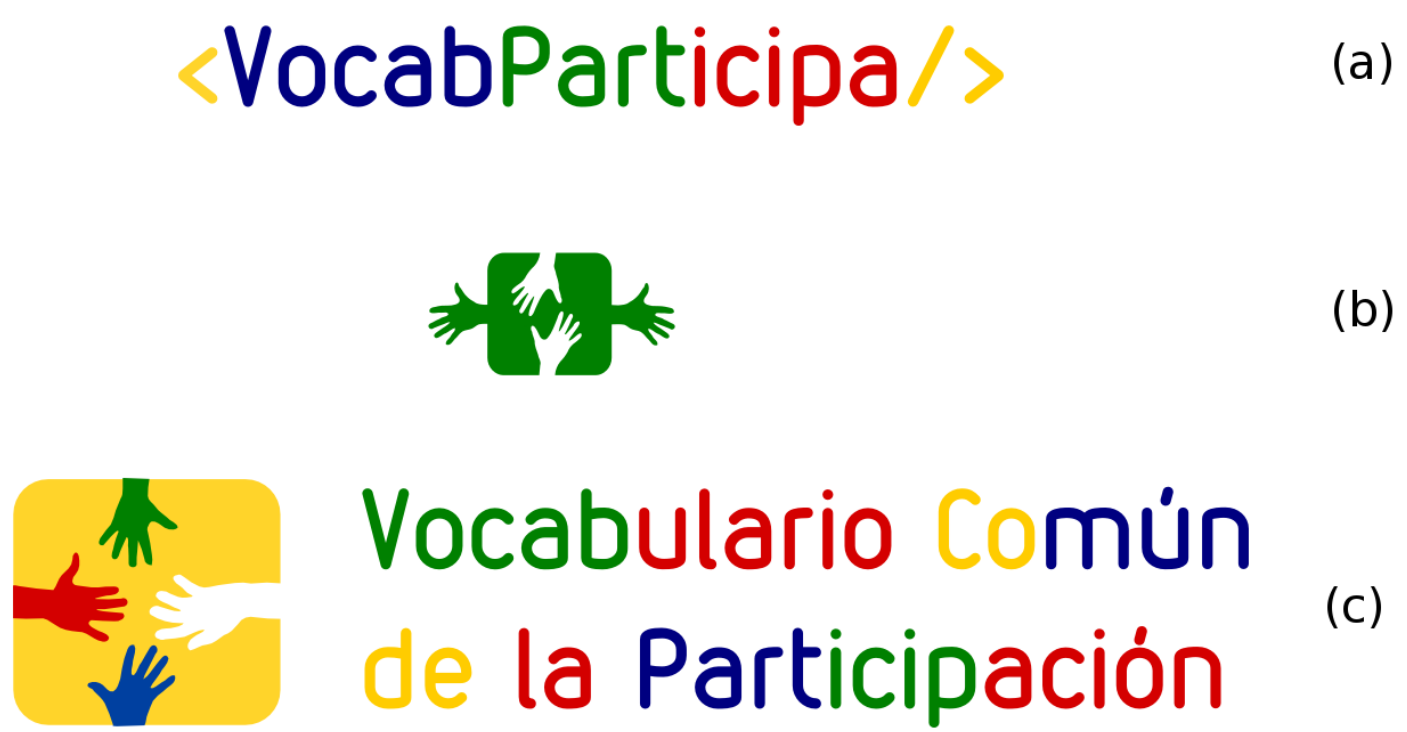
\includegraphics[width=0.4\textwidth]{figs/logoUnificadoDoPDF}
    \caption{Some of the various logos for the OSP. (a) is a colored text logo proposal; (b) is a figurative logo; (c) is mixture of both ideas. It can be seen that these logos were conceived for the ontology when it was called a \emph{vocabulary}. Community documents reflect this nomenclature, which is being changed with this article and subsequent work.}
    \label{logo}
\end{figure}


%\begin{figure}[hb]
%    \centering
%    \includegraphics[width=0.2\textwidth]{figs/logo3}
%    \caption{A figurative logo for the Common Vocabulary of Social Participation. There are dozens of variants of this logo, black and white, RGBY colored, mixed with text, etc. See figure~\ref{logo} for a textual version, and figure~\ref{logo3} for a mixture.}
%    \label{logo2}
%\end{figure}
%
%\begin{figure}[hb]
%    \centering
%    \includegraphics[width=0.2\textwidth]{figs/logo2_vocab_participa}
%    \caption{A logo with text and figure, a mixture of logos in figures~\ref{logo} and~\ref{logo2}, with Spanish text.}
%    \label{logo3}
%\end{figure}
%



\subsection{OWL code of CVSP}\label{owl}

The OWL code for the CVSP is online~\cite{owlVcps}. 
% Estou voando nas alturas
The CVSP OWL code did not contain all relation from Figure~\ref{fig:v1}. This is directly addressed in Section~\ref{exp}, which exposes the implementation of all relations in the OSP, including CVSP OWL corrections and adjustments to best practices. The complete and correct OSP ontology is then expanded in Section~\ref{downwards}.
A diagram representation OSP taxonomy is presented in Figure~\ref{fig:vcpsCC}, while the ontology diagram is at Figure~\ref{fig:v1}.

\subsection{Blog Posts}
The CVSP blog~\cite{coraisBlog}
aggregates both important discussions and documents in no more than twenty posts to date.
All OWL code, final documents, public consultations, mental map and images are posted in the blog~\cite{coraisBlog}. 
The first post was in July 24, 2012. Last post to date is from May 7, 2013.
Most blog posts are from the first day (almost half of them). They received more than
twenty commentaries. Two ``out-of-season'' blog posts, one in August 9, 2012 and another in October  22, 2012, separate first day posts from last posts. Both have about ten commentaries.
Last blog posts occurred as a few days burst and a final message, a month after.

There are three more recent blog posts, from November and December, 2013. But these already address OPS conception from CVSP.

\subsection{Discussions and etherpads}
There are numerous commentaries in the blog posts, in which collective elaboration was registered. Besides that, four etherpads 
were written (these are interfaces that allows writting online texts with multiple simulteneous contributors~\cite{etherpads}):
\begin{itemize}
    \item A pad for important words.
    \item A pad dedicated to a second phase of the common vocabulary elaboration, which did not happen yet.
    \item A pad for process documentation. It became the first document described in Subsection~\ref{refDocs}. 
    \item A pad for both vocabulary specification and ``questions not addressed to in the webinar''.
\end{itemize}



\section{OSP: the Ontology of Social Participation}\label{exp}
%A pr�xima secao j� � a conclus�o. Alem dessa sess�o ter ficado grande, voce precisa uma sess�o onde demonstra que essa ontologia � util para alguma coisa

\begin{figure*}
    \centering
    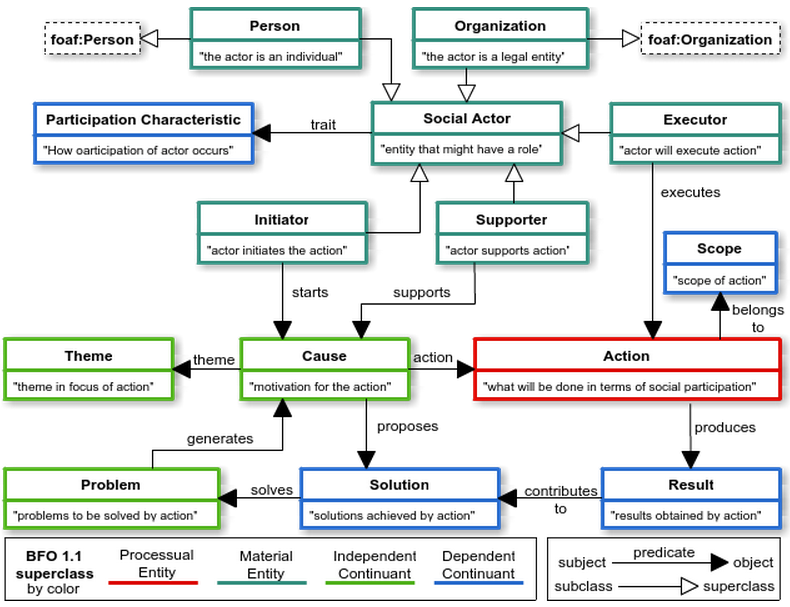
\includegraphics[width=0.9\textwidth]{figs/opsBFO___}
    \caption{Diagram representation of the Ontology of Social Participation (OSP). Arrows with white heads indicates ``is a'' relations (subclass points to superclass). Arrows with black heads indicates property relations from subject to object . All property relation yield existential restrictions, with the exception of the ``has characteristic'' property, that does not yield restriction.}
    \label{fig:v1}
\end{figure*}

 
Followng the exposition in Section~\ref{sec:into}, from the CVSP the OSP was conceived. This section makes four considerations about OSP: first is label standardization and an exhibition of implemented and unimplemented CVSP classes, properties and restrictions. Features present in Figure~\ref{fig:v1}, but not present in the community release, are fully implemented in Section~\ref{impl}. Elementary further specification of subclasses is addressed in Section~\ref{downwards}. Examples of usage are addressed in subsection~\ref{examplesUsage}. 

For completeness of exposition and deference to CVSP community efforts, consideration of upper ontologies is at Subsection~\ref{upper} and the public consultation model depicted in Figure~\ref{fig:consult} is considered at Subsection~\ref{public}. 

\subsection{Standardization and exhibition of implemented features}\label{impl}
Without explicit criteria, CVSP IRI was \url{http://lumii.lv/ontologies/Corais.owl}. OPS IRI was chosen to be \url{http://purl.org/socialparticipation/ops} for the following reasons:
\begin{itemize}
    \item This IRI is directly related to the ontology name (OPS).
    \item This IRI, also an URL, is independent from government and other political parties. This is important to coalesce with interested parties: the Brazilian Federal Social Participation Portal\cite{participa}, Brazilian government repository of vocabularies and ontologies~\cite{vocab}, civil society and NGOs.
    \item The IRI, when reached via HTTP, can be redirected to where current documentation is held.
\end{itemize}

Labels in the languages of interest should be written in label fields. Even so, class names can be friendly to (potential) users, bearing the attention not to take the class name as the label or as a meaning restriction.

For standardization, all classes were written in CamelCase and without accents. Class names were written in English to ease internationalization, adoption and maturation. Labels were written in Portuguese, English and Spanish. Therefore, class names changed, receiving respective labels and a plain textual short explanation.
Table~\ref{ospClasses} exhibits all classes is OSP.

\begin{table*}
    \footnotesize
  \centering
  \caption{Classes of the OSP (Ontology of Social Participation). These are core concepts in the ontology. Along with the taxonomic structure exposed in Figure~\ref{}, these classes are related by the properties in Table~\ref{ospProps}.}
  \begin{tabular}{|l|l||p{2.2cm}|p{2.2cm}|p{1.8cm}||p{4cm}|}\hline
{\bf OSP class name} & {\bf CVSP class name} & {\bf pt-br label} & {\bf es label} & {\bf en label} & {\bf definition} \\\hline\hline
Problem & Problema & Problema & Problema & Problem & the problem that the Action aims to solve \\\hline
Result & Resultados & Resultado & Resultado & Result & the result obtained with action realization \\\hline
Theme & Tema & Tema & Tema & Theme & the theme in focus by action \\\hline
Cause & Causa & Causa & Causa &  Cause & the motivation for the execution of the action \\\hline
Action & Acao & A\c{c}\~ao & Acci\'on & Action & what is done in terms os social participation \\\hline
Solution & Solucao & Solu��o & Soluci\'on & Solution & solucion achieved with the action \\\hline
ParticipationCharacteristic & NivelDeParticipacao & Caracter\'istica de Participa\c{c}\~ao & Caracter\'istica de Participaci\'on & Participation Characteristic & the way the participation of s specific actor, is happening \\\hline
ActionScope & Espa\c{c}o de A\c{c}\~ao & Escopo de A\c{c}\~ao & Ambito de Accio\'on & Action Scope & the scope os Action execution \\\hline
Role & Papel & Papel & Rol & Role & the role of the actor \\ \hline
Supporter & Apoiador & Apoiador & Apoyador & Supporter & supports cause with resources of any kind (e.g. cognitive, financial, equipments) \\ \hline
Initiator & Iniciador & Iniciador & Iniciador & Initiator & originates cause, individually or collaborativelly \\ \hline
Executor & Executor & Executor & Ejecutor & Executor & performs action directly and is responsible for results \\ \hline
SocialActor & Ator & Ator Social & Actor Social & Social Actor & entity that might have a role \\ \hline
Organization & Organizacao & Organiza\c{c}\~ao & Organizaci\'on & Organization & social actor is a group of individuals, organized formally or informally (e.g. movements, collectives) \\ \hline
Person & Pessoa & Pessoa & Persona & Person & a person (social actor is a person) \\ \hline
  \end{tabular}
  \label{ospClasses}
\end{table*}

OSP Properties fit headlessCamelCase format, are readable in English (to ease internationalization, adoption and maturation), and have well defined domains and ranges. Table~\ref{ospProps} is dedicated to OSP properties, with labels in English, Portuguese and Spanish.

\begin{table*}
    \footnotesize
  \centering
  \caption{Properties of the OSP (Ontology of Social Participation).}
  \begin{tabular}{|l|l||p{2.2cm}|p{2.2cm}|p{1.8cm}||l|p{2.2cm}|}\hline
{\bf OSP property name} & {\bf CVSP property name} & {\bf pt-br label} & {\bf es label} & {\bf en label} & {\bf domain} & {\bf range} \\\hline\hline
hasTheme & possuiTemaAssociado & possui tema & contiene tema & has theme & Cause & Theme \\ \hline
belongsToScope & pertenceAoEspaco & pertence ao escopo & pertence al campo & belongs to scope & Action & ActionScope \\ \hline
hasRole & temPapel & possui papel & tener rol & has role & SocialActor & Role \\ \hline
supportCause & apoiaCausa & apoia causa & apoya causa & supports cause & Supporter & Cause \\ \hline
composesSolution & compoeSolucao & comp\~oe solu\c{c}\~ao & componer soluci\'on & composes solution & Result & Solution \\ \hline
executesAction & executaAcao & executa a\c{c}\~ao & ejecuta acci\'on & executes action & Executer & Action \\ \hline
generatesCause & geraCausa & gera causa & genera causa & generates cause & Problem & Cause \\ \hline
startsCause & iniciaCausa & inicia causa & ainicializa causa & starts cause & Initiator & Cause \\ \hline
solvesProblem & soluciona & soluciona problema & resuelve problema & solves problem & Solution & Problem \\ \hline
hasAction & possuiAcao & possui a\c{c}\~ao & tiene acci\'on & has action & Cause & Action \\\hline
producesresult & produzResultado & produz resultado & producir resultado & produces result & Action & Result \\\hline
proposesSolution & propoeSolucao & prop\~oe solu\c{c}\~ao & propone soluci\'on & proposes solution & Cause & Solution \\\hline
hasParticipationCharacteristic & temNivelDeParticipacao & possui caracter\'istica de participa\c{c}\~ao & tiene caracter\'istica de participaci\'on & has participation characteristic & Role & ParticipationCh-aracteristic \\\hline
  \end{tabular}
  \label{ospProps}
\end{table*}

All restrictions in OSP are existential and all properties yield restrictions, except hasParticipationCharacteristic. Table~\ref{ospRestr} is dedicated to OSP restrictions.

\begin{table}
  \centering
  \caption{Restrictions of the OSP (Ontology of Social Participation). All OSP restrictions are existential (\texttt{owl:someValuesFrom)}.}
  \begin{tabular}{|l|l|l|}\hline
{\bf subject} & {\bf predicate} & {\bf object} \\\hline\hline
Initiator    & startsCause        & Cause\\\hline
Supporter    & supportsCause      & Cause\\\hline
Executer     & executesAction     & Action\\\hline
Solution     & solvesProblem      & Problem\\\hline
SocialActor  & hasRole            & Role\\\hline
Action       & producesResults    & Results\\\hline
Result       & composesSolution   & Solution\\\hline
Cause        & dasAction          & Action\\\hline
Action       & belongsToScope     & Scope\\\hline
Cause        & hasTheme           & Theme\\\hline
Cause        & proposesSolution   & Solution\\\hline
Problem      & generatesCause     & Cause\\\hline
  \end{tabular}
  \label{ospRestr}
\end{table}

It is important to realize that OSP is dedicated to a complete social participation process, with a beginning, middle and end.
Thus, such OWL restrictions are valid for the final state of the process (for example, in an arbitrary snapshot, a \texttt{SocialActor} may be not tied to a role). This might lead to NULL or ``not yet defined'' field supplies.

A comparison of the CVSP OWL code~\cite{owlCCPtg} 
with the diagram in Figure~\ref{fig:v1}, which reflects official CVSP documentation, revealed that a class, two properties and three restrictions were not implemented. These were fully implemented in OPS. These are the missing classes, properties and restrictions missing in CVSP and that were implemented in OSP:

\begin{itemize}
    \item Class: ParticipationCharacteristic.
    \item Property: hasRole.
    \item Property: composesSolution.
    \item Restriction: Role hasParticipationCharacteristic some ParticipationCharacteristic.
    \item Restriction: Results composesSolution some Solution.
    \item Restriction: Problem generatesCause some Cause.
\end{itemize}

Also, in CVSP, existential restrictions were  written as ``min 1''. 
These were changed to the standard ``some'' existential restriction.

OSP is available online~\cite{owlOSP}. To ease navigation of the ontology by interested parties, it is also available in the Webprotege interface~\cite{owlOSPwp}. The diagram of OSP taxonomic structure is exposed in Figure~\ref{fig:owlCC}.

Examples of upper ontologies usage with OSP is under development and should be available in a dedicated work, as possibilities should be inspected carefully. Pertinent to OSP, but not upper ontologies, are FOAF~\cite{foaf} (for describing people and things they do) and Dublin Core~\cite{dublin} (for describing resources, with special attention to digital resources).

\subsection{OSP growth}\label{downwards}

\begin{figure*}
    \centering
        \includegraphics[width=2\columnwidth]{figs/cospExp}
    \caption{A taxonomic diagram of an expanded instance of OSP. Darker orange marks defined classes: PaidExecutor is defined as being the subject of a \texttt{receivesFrom} relation with a \texttt{SocialActor}; \texttt{DownloadedMob} is defined by being the subject of a \texttt{convoquedBy} relation with a \texttt{SocialNetwork}. OWL code is online for live editing~\cite{owlExp}. The new classes added to OSP are in Table~\ref{ospFooClass}}
    \label{fig:owlExp}
\end{figure*}

To this point, OSP is complete (no missing classes, properties and restrictions with respect to documentation), correct (no spaces in URIs and \texttt{min 1} restrictions specified as existential restrictions), and names of classes and properties standardized (English in CamelCase and headlessCamelCase). This way, OSP matches, with coherence, CVSP community online documentation~\cite{corais}. As no greater consensus was reached, further developments of OPA should wait feedback and unroll of community processes.

As an example of possible aditional classes, another instance of the ontology is uploaded to Webprotege, from which some newly created classes and properties are exhibited~\cite{owlExp}. Table~\ref{ospFooClass} is dedicated to these aditional classes while Figure~\ref{fig:owlExp} exhibits the resulting taxonomic structure.

The property \texttt{receivesFrom} was also added and has an inverse: \texttt{SocialActor ``paysTo'' Executor}. Also, the \texttt{DownloadedMod} class is a defined class by the restricton: \texttt{Mob convoquedBy Network}, with a newly defined property \texttt{convoquedBy}.

This is one of the numerous ways by which OSP might deal with further classes, properties and restrictions. This particular expansion was chosen as an example by plain observance of community documentation and recent social affairs, such as the Brazilian protests.

\begin{figure}
    \centering
    \includegraphics[width=\columnwidth]{figs/cospTax}
    \caption{A taxonomic diagram of the Ontology of Social Participation (OSP). This image was rendered inside Protege, with the OWL code in Appendix~\ref{owl:vcps}.}
    \label{fig:owlCC}
\end{figure}

\begin{table*}
  \centering
  \caption{New classes considered for expansion of the OSP. The taxonomic organization of these classes, within OSP can be oberved in Figure~\ref{fig:owlExp}. Further information is in Section~\ref{downwards}.}
  \begin{tabular}{|l|l|p{5cm}|p{5cm}|}\hline
{\bf new class} & {\bf subclass of} & {\bf description} & {\bf further notes} \\\hline\hline
SocialNetwork & Organization & a social structure made up of social actors (such as individuals or organizations) and a set of dyadic ties between these actors & --//--\\\hline
FreeScaleNetwork & SocialNetwork & a network whoose connectivity follows a power law & disjoint with UniformrandomNetwork and GeographicNetwork \\ \hline
UniformRandomNetwork & SocialNetwork & also known as Erd\"os Renyi network, this network sets, with equal propability, an edge between each pair of nodes & disjoint with FreeScaleNetwork and GeographicNetwork\\\hline
GeographicNetwork & SocialNetwork & a network whose connectivity is related to the distance of nodes in a metric space & Disjoint with both FreeScaleNetwork and UniformRandomNetwork \\\hline
SmallWorldNetwork & SocialNetwork & a network where most nodes can be reached from other nodes with few hops or steps & not disjoint with FreeScaleNetwork, UniformNetwork and GeographicNetwork\\\hline\hline
InformalOrganization & Organization & an organization that is not formalized & disjoint with Intitution \\ \hline
Mob & InformalOrganization & a crowd of individuals & --//-- \\\hline
GiantMob & Mob & a crowd with more than 10,000 individuals & --//--\\\hline
DownloadedMob & Mob & a Mob convoqued by a network & this is a defined class, by being a network and being the subject of the relation convoquedBy with object Network \\ \hline\hline
Institution & Organization & a mechanism of social order that governs a set of individuals & disjoint with InformalOrganization \\\hline
PublicInstitution & Institution & an institution backed through public funds and controlled by the state & disjoint with Private Institution \\ \hline
PrivateInstitution & Institution & an institution backed through private fundings and controlled by private parties & disjoint with PublicInstitution \\ \hline
AcademicInstitution & Institution & an institution dedicated to education and research, which grants academic degrees & --//-- \\ \hline
NGO & Institution & a legally consituted corporation created by natural or legal people that operate independently from anu form of government & --//-- \\\hline
SpuriousInstitution & Institution & an institution that holds prominent illegitimate or corrupt characteristcs & --//-- \\\hline
ExoticInstitution & Institution & and institution that does not fir previous classes or is characterized by a very unique traces & --//-- \\\hline\hline
VoluntaryExecutor & Executor & an executor that receives no formal reward for the tasks & disjoint with PaidExecutor \\ \hline
PaidExecutor & Executor & an Executor that receives formal reward for the tasks accomplished & a defined class, being an Executor and the subjecto of a receivesFrom predicate with SocialActor as object\\ \hline
  \end{tabular}
  \label{ospFooClass}
\end{table*}
%\subsubsection{SparQL examples of usage}

\section{OSP utility}\label{ospUtil}
OSP is meant to be useful. First, as a sistematization of what is social participation to Latin America groups, as conceived by CVSP. Second, as a mean to ease linked data, and enable integration of various instances for social participation. An indicative of this pertinence is OPA, an ontology that already uses OSP.



\subsection{Usage of OSP via a SparQL endpoint}
Accessing multiple databases is one of the OWL ontology basic purposes. The standard way to acess these data via ontologies is by using a SparQL endpoint. This endpoint delivers data from a triplestore or, with more experimental technology, relational database systems, such as a MySQL server (e.g. via OnTop/Quest~\cite{onTop}). Either way, the query is the same, i.e. the user or machine reaching the endpoint uses the same protocol in order to retrieve information through semantic criteria. Figure~\ref{endpoint} is a schematic representation of OBDA (Ontology Based Database Access), which is a common name for this multiple database access through ontologies.

\begin{figure}
    \centering
        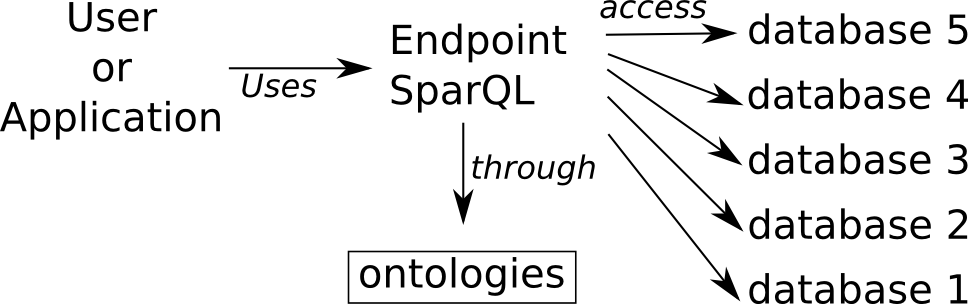
\includegraphics[width=0.9\columnwidth]{figs/endpoint}
    \caption{Scheme of the common use of ontologies for multiple databases integration. A user or application reaches a SparQL endpoint. This endpoint, throught ontologies, delivers data from one or more databases. Nowadays, the most usual is to find only one database available in an endpoint, and this database is usually duplicated and not synchronized, but available as a (converted) triplestore. Even so, it is possible to access multiple ontologies and it is desirable that the databases have synchronous access, i.e. without need to convert data to triples beforehand.}
    \label{endpoint}
\end{figure}

Some examples of this usage can be given by SparQL queries and concise explanations:
\begin{itemize}
    \item \texttt{"select ?s ?s2 ?s3 where \{?s a ops:SocialActor . ?s2 a ops:Person . ?s3 a ops:Organization\}"}: this query retrieves all social actors (\texttt{?s}), be each a person or an organization, all persons (\texttt{?s2}) and all organizations (\texttt{?s3}). In a similar manner, one can retrieve all roles played, all executers, all initiators and all supporters.
    \item \texttt{"select ?s ?o where \{?s ops:startsCause ?o\}"}: this query retrieves all causes started and their initiators.
    \item \texttt{"select ?s ?s2 ?o ?o2 where \{ ?s a ops:Action . ?s ops:belongsToField ?o . ?s2 ops:executesAction ?s . ?s ops:producesResults ?o2\}"}: this query retrieves all actions (\texttt{?s}) along their Action Field (\texttt{?o}), their Executer (\texttt{?s2}) and their Results (\texttt{?o2}).
\end{itemize}

\subsection{Discursive examples of usage}\label{examplesUsage}

OSP usage might not be obvious at first. How is data being linked? How is field knowledge being organized? Core principles of this utility, reflecting the exposition in Section~\ref{sec:into}, can be understood by the following observations:
\begin{itemize}
    \item Different participation instances have social actors, actions being developed, organizations involved, problems being tackled, etc. These can yield one consistent database by means of OSP usage.
    \item One can understand the mutually exclusive nature of being a paid or a voluntary contributor by observing the expanded version of OSP, exposed above. Also, noticing the fact that a mob can be very big or not, and that it can be convoqued or not by a Network, can make the field more neat for a newcommer or ease discussions and problematizations for senior researchers or politicians.
\end{itemize}

Imagined examples are useful to make these points clear:
\begin{itemize}
    \item Suppose a public SparQL endpoint unifies several participation instances by means of OSP. Thus, the number of participants (Social Actors) is publicly available. Also, depending on the platforms, one can observe how many are individuals, how many are organizations, and understand to which extent the corporative influence is explicit. One can observe how many of the participants are the same in each platform, and what roles they take, and make conclusions about how much society is really participating or if these processes are manipulated by the same agents. One can also gaze uppon the problems being discussed and which solutions are being proposed, therefore easing the sense of what is being considered important and valid as public discussions. This list of possibilities is endless, specially when OSP variations and expansions are considered.
    \item Suppose a person, say Jessica, has a new proposal for a participative system that uses OSP. She can have a quite concise understanding of the concepts involved, and how they relate, by means of OSP. She can now make very objective observations and deliver clear suggestions that relate directly to the system being used. She can even make an OSP variation or another ontology, as a way to confront the schemes.
    \item Supose there is an automatic system for exhibiting indicators about social participation (how effective it has been, how wide the scope of interests, etc). Instances that are integrated by OSP are queried for information and, for example, this system registers any organization involved as a social actor. In the case of the expanded OSP exposed above, for example, the system registers any mob, whose incidence was recorded in the database as a \texttt{DownloadedMob}, as related to some social network, be the network known or not.
\end{itemize}


\section{Concluding remarks and future work}\label{conc}
OSP, based in CVSP, % Essa aqui? Mesmo que voce decida usar o mesmo nome para as duas, vai ter que fazer algo OSP 1 e OSP 2 para separar as duas de forma a n�o haver mais confus�o.
yields initial steps in achieving an effective social participation ontology: community has registered activities and delivered reference documents, including the OWL ontology presented in this article. If on one hand such an ontology is difficult to be obtained in short term, on the other hand this is a precedent in which deeper observations can take place.

Sections~\ref{ospUtil},~\ref{downwards},~\ref{upper} and~\ref{public} have expansion directions for the ontology, regarding uses, further definition of classes, upper ontologies and related ontologic structures.

On the practical side, the use of this ontology or related developments for the Brazilian federal participation portal (\url{Participa.br}~\cite{participa}) is a desirable possibility, as it implies usage and good maintenance. The parties responsible for such portal and for Brazilian government vocabularies and ontologies have already taken a step towards this development, with direct contact with authors and the publication of OSP in a government instance~\cite{pubVocab}. Moreover, an ontology was done for \url{Participa.br}, based in the OSP~\cite{opa}. This is confluent with the presidential Decree that establish a policy and commitment for social participation\cite{decree}. In this context, presidential and ministerial parties have come close, to start formalizing current legal participatory mechanisms (e.g. conferences, forums, roundtables) in ontological terms.
Hosting of ontologies on Webprotege~\cite{webprotege} have become central, as a way to share specific ontologies and collects commentaries.

\subsection{Further work}
Further works involves observing community manifestations about OSP and this article, accomplishing use by means of formal instances and civil society, studying upper ontologies usage with OSP and creating new ontologies for each Brazilian formal social participation instances (e.g. ombudsman office, roundtables, councils, foruns, conferences). The use of OSP (or a variant) in different instances is envisioned for creating indicatives of social participation and easing participation processes, which should be better studied.

Future work involves careful consideration of Basic Formal Ontology to enhance linking participation data to scientific research. 
Also, further detailing subclasses might be carefully modeled for different instances, with respective interested parties. 


\begin{figure*}
    \centering
    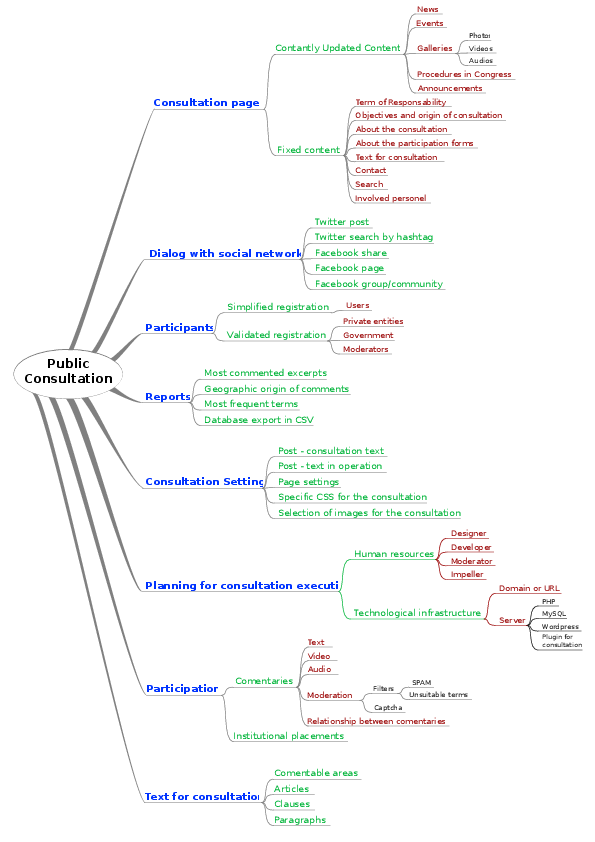
\includegraphics[width=0.9\textwidth]{figs/publicConsultation__}
    \caption{A diagram representation of a general public consultation. The OWL implementation of this model is in subsection~\ref{public}.}
    \label{fig:consult}
\end{figure*}



\begin{acknowledgments}
This article is heavily influenced by Protege and BFO documentation. Authors thank community and researchers related to these projects~\cite{protege,bfo}.
Renato Fabbri is grateful to CNPq (project 870336/1997-5) and 
the Postgraduate Committee of the IFSC/USP.
Authors thank Silvio Domingos Cardoso.
\end{acknowledgments}


\appendix

\section{Upper and domain ontologies}\label{upper}
There are various ontologies of interest for participatory democracy. To exemplify, three upper ontologies were chosen:
\begin{itemize}
    \item BFO $\rightarrow$ the Basic Formal Ontology is oriented to scientific use of data, which is confluent with Brazilian hackers and scientific community~\cite{bfo}. 
    \item DBpedia $\rightarrow$ ``a crowd-sourced community effort to extract structured information from Wikipedia''. Convenient for bootstrapping the OPS to out-of-domain knowledge with crowd-sourced structured information~\cite{dbpedia}.
    \item W3C recommendations for open-government, these are the work product of specialized groups and are regarded in high account by the semantic web community~\cite{egovW3C}.
\end{itemize}

\section{Public consultation}\label{public}
Public consultations have core importance in participatory democracy and the model in figure~\ref{fig:consult} was conceived as part of OSP community documentation.
Therefore, an OWL implementation of such public consultation, should be developed and made public, with dedicated attention.
Considerations of this public consultation with respect to the OSP and formal existent instances should be addressed as well.
This public consultation model is observed here for completeness of exposition and further details goes beyond the scope of this article.



\section{OWL code of the Ontology of Social Participation}
\label{owl:vcps}


\lstinputlisting[language=owlms]{rdf/ops.ttl}
\nocite{*}
\bibliography{paper}% Produces the bibliography via BibTeX.

\end{document}
%
% ****** End of file aipsamp.tex ******
